\chapter{Simulation}

%--------------------------------------------------------------------------------------------------------
% 		Intro
%--------------------------------------------------------------------------------------------------------
\section{Intro}

This will be used to test the performance of message ferrying algorithm using parametric studies.  

The speed of the ferries is random and the direction is random, where the speed is within 36kph to 72kph in a uniform distribution.  

In this section, we examine the performance evaluations of message ferrying design to focus on two parameters.  
One of the parameters is to determine a so-called packet loss where we measure the buffer size limit versus the packet dropping threshold within ferries.
Because of the nature of the algorithm, there may be dropped packets when the update number is older.
This packet loss is defined as where it measures the number of packets dropped when the buffer is full, and the oldest packets are dropped to accommodate for adding the new packet.  
We define our packet loss as the number of packets dropped due to the fact that the buffer size limit has been reached.
In this scenario, to test our design implementation, a simple scenario is created to validate that the node models are working as designed.  
The other is to find the delay, which is measured by the time to update the central repository.
%More realistic scenario
%	- Random ferry movement
%		- Details -> car
%	- even source spacing

%--------------------------------------------------------------------------------------------------------
% 		Topology
%--------------------------------------------------------------------------------------------------------
\section{Network Model}

In Figure \ref{fig:scenario2}, our scenario for the packet .  The size of this topology is 1km x 1km.  
That is the distance between source node 0 and 4 is 1km, while the distance between source node 6 and 2 is also 1km.  
The speed of the ferries is random and the direction is random, where the speed is within 36kph to 72kph in a uniform distribution.  

%overview of the scenario2 (random movement)
\begin{figure}[h]
    \centering
    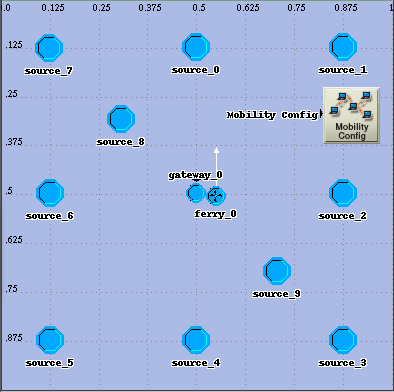
\includegraphics[width=.5\textwidth]{images/scenario2-top}
    \caption{Topology of Scenario 2}
    \label{fig:scenario2}
\end{figure}

%Might not need subsections for Scenario 1 & 2

\subsection{Scenario 1}

%1 gw, 1 ferry

\subsection{Scenario 2}

%2 gw, 2 ferry

\subsection{Common Settings}

%Characteristics of random ferry movement
%	- Speed 
%	- Beaconing intervals
%	- Property update interval


%--------------------------------------------------------------------------------------------------------
% 		Metrics and Results of Interest 
%--------------------------------------------------------------------------------------------------------
\section{Metrics and Results of Interest }

%Some introduction

\subsection{Success Rate and Loss}
%Result of Interest 1: Success rate
%	- Main parameter of interest affecting success rate -> memory size
%	- Need to talk about what constitutes success rate

\subsection{Delay}
%Result of Interest 2: Delay
%	- Main parameter of interest affecting delay -> number of ferries & gateways
%	
%Something about delay for lost packets

\subsection{Parameters Varied} %TODO: better section title

The following factors have been considered when designing scenarios:
\begin{itemize}
\item Number of sources to ferries to gateways (various ratios)
\item Speed and trajectories of ferries (random vs set path)
\item Rate of source node state changes
%\item Buffer size of ferries and size of property values (affects packet sizes)
%\item Distances and distributions of ferries and gateways
\end{itemize}

\subsubsection{Memory Limit}
In the following graph, we can see that the buffer size used is proportional to the rate of successful packets delivered to ferries.
%graph of results for buffer size vs. packet loss [uncomment this when ready]
%\begin{figure}[h]
%    \centering
%    \includegraphics[width=.5\textwidth]{images/result1}
%    \caption{Buffer size versus packet drop rate }
%    \label{fig:result2}
%\end{figure}
This result was what we expected.  
The increase of the buffer size used resulted in fewer packet dropouts.

\subsubsection{Number of Ferries and Gateways}
%See topology section
%gateway scenario
The increase of the number of gateways reduced the delay of updating to central repository.  
This result was expected because we knew that by properly placing another gateway in the area will grant better coverage.  
\subsection{Seed - Effect of Randomness}

\subsection{Source Node Storage}
